\documentclass[a4paper]{article}
\usepackage{digitalspeech}
\usepackage{amssymb,amsmath,amsfonts,graphicx}
\usepackage[english]{babel}
\usepackage{graphics}
\usepackage{epsf,psfig}

\ifpdf
\DeclareGraphicsExtensions{.pdf,.jpg,.tif}
\else
\DeclareGraphicsExtensions{.eps,.pdf,.jpg,.tif}
\fi

\title{AMT3D: Extending Acoustic Multi-Target Tracking from 2D to 3D Space}

\name{Roee Douek}

\address{
roee.douek@campus.technion.ac.il\\
Technion - Israel Institute of Technology}

\begin{document}
\maketitle

\begin{abstract}
{\ninept This work presents AMT3D, an extension of the AMT+ acoustic multi-target tracking system from two-dimensional to three-dimensional space. The transition from 2D to 3D tracking introduces fundamental challenges including geometric ambiguity in the vertical dimension, increased computational complexity for multi-ellipsoid intersections, and reduced precision in z-axis measurements. We address these challenges through enhanced state modeling with 9-dimensional vectors, adaptive noise handling for vertical measurements, and improved ellipsoid intersection algorithms. Performance evaluation across three microphone array configurations demonstrates the feasibility of 3D acoustic tracking with mean tracking errors ranging from 0.095 m to 0.192 m depending on noise conditions and array geometry. The implementation provides a foundation for extending acoustic tracking applications from planar to full 3D environments.}
\end{abstract}

\section{Introduction}

\subsection{Background: AMT+ 2D System}

The AMT+ (Acoustic Multi-Target Plus) system \cite{amt_plus} established a foundation for acoustic multi-target tracking using smartphone-based MIMO arrays. The original system operates in 2D space and achieved significant advances over previous acoustic tracking approaches.

\subsubsection{AMT+ Signal Foundation}

AMT+ employs Zadoff-Chu (ZC) sequences as the signal foundation, which provides several critical advantages:

{\bf ZC Sequence Properties:}
\begin{itemize}
\item {\em Constant Amplitude:} ZC sequences maintain constant amplitude, optimizing signal power utilization
\item {\em Zero Auto-correlation:} Perfect auto-correlation properties enable precise timing detection
\item {\em Weak Cross-correlation:} Different ZC sequences exhibit minimal cross-correlation, enabling source separation
\end{itemize}

The ZC sequence is mathematically defined as:
\begin{equation}
z[n] = \begin{cases}
e^{-j2\pi u/N_{zc} \cdot (n(n+1)/2 + qn)} & \text{for } N_{zc} \text{ odd} \\
e^{-j2\pi u/N_{zc} \cdot (n^2/2 + qn)} & \text{for } N_{zc} \text{ even}
\end{cases}
\label{eq:zc_sequence}
\end{equation}

where $N_{zc}$ is the sequence length, $u$ is a root index with $\gcd(u, N_{zc}) = 1$, and $q$ is an integer parameter.

\subsubsection{AMT+ Algorithm Flow}

The AMT+ system implements a sophisticated 5-stage processing pipeline:

{\bf Stage 1: Source Separation}
\begin{itemize}
\item {\em MIMO Signal Processing:} Each microphone receives mixed signals from multiple speakers
\item {\em Self-Interference Cancellation:} Actively removes interference from other speakers using estimated channel responses
\item {\em Sliding-Window Correlation:} Exploits ZC sequence properties for signal separation
\end{itemize}

{\bf Stage 2: Direct Signal Detection}
\begin{itemize}
\item {\em Correlation-Based Detection:} Identifies direct path arrival as maximum correlation peak
\item {\em Phase Offset Correction:} Refines timing using phase analysis to achieve sub-sample accuracy
\item {\em Time Synchronization:} Establishes precise sender-receiver timing alignment
\end{itemize}

{\bf Stage 3: Interference Elimination}
\begin{itemize}
\item {\em 4th-Order MTI Filter:} Moving Target Indicator filter removes static reflections: $h_{MTI}(n) = \delta(n) - 4\delta(n-N) + 6\delta(n-2N) - 4\delta(n-3N) + \delta(n-4N)$
\item {\em Adaptive Thresholding:} Dynamic noise floor estimation: $Th = \text{mean}(D) + k \cdot \text{std}(D)$
\item {\em Consecutive Subtraction:} Removes static object influences
\end{itemize}

{\bf Stage 4: Primary Echo Detection}
\begin{itemize}
\item {\em Non-Particle Target Modeling:} Recognizes targets as extended objects, not point sources
\item {\em Primary Echo Identification:} Detects the fastest-moving point (e.g., fingertip) among multiple target reflections
\item {\em Distance Projection Analysis:} Uses unique reflection patterns for target characterization
\end{itemize}

{\bf Stage 5: Multi-Ellipse Localization}
\begin{itemize}
\item {\em Ellipse Construction:} Each speaker-microphone pair creates a ranging ellipse with path length equal to measured echo time
\item {\em Multi-Target Identification:} Distance projection patterns enable continuous target tracking
\item {\em 2D Position Estimation:} Intersection of multiple ellipses determines target locations in planar space
\end{itemize}

\subsubsection{AMT+ Tracking Approach}

The original AMT+ system performs **position-only tracking** in 2D space using multi-ellipse intersection. Key characteristics include:

\begin{itemize}
\item {\em Position Tracking:} Estimates current 2D position (x, y) without explicit velocity or acceleration modeling
\item {\em Ellipse Intersection:} Uses geometric intersection of ranging ellipses for localization
\item {\em Distance Projection:} Employs unique reflection patterns for multi-target identification and continuous tracking
\item {\em Particle vs Non-Particle:} Recognizes targets as extended objects rather than point sources
\end{itemize}

\subsubsection{AMT+ Performance Achievements}

The original AMT+ system demonstrated exceptional performance in 2D tracking:

\begin{itemize}
\item {\em Single Target:} 0.54 cm average tracking error
\item {\em Dual Target:} 1.37 cm average tracking error  
\item {\em Triple Target:} 2.13 cm average tracking error
\item {\em Gesture Recognition:} 97.0\% classification accuracy for 14 gesture types
\item {\em Processing Delay:} Less than 80 ms for real-time operation
\end{itemize}

\subsection{Motivation for 3D Extension}

Real-world acoustic tracking applications require full three-dimensional capabilities:

\begin{itemize}
\item {\em Human Activity Monitoring:} Tracking body movement, gesture recognition, and posture analysis
\item {\em Drone/UAV Tracking:} Monitoring aerial vehicles in indoor environments
\item {\em Smart Home Applications:} Room-scale interaction and presence detection
\item {\em Industrial Monitoring:} Equipment and personnel tracking in 3D factory spaces
\end{itemize}

However, extending from 2D to 3D introduces significant technical challenges that cannot be solved by simply adding a third dimension to existing algorithms.

\subsection{AMT3D System Architecture}

Figure \ref{fig:system_architecture} illustrates the AMT3D system architecture, showing the key components developed for 3D extension.

\begin{figure}[t]
\centerline{
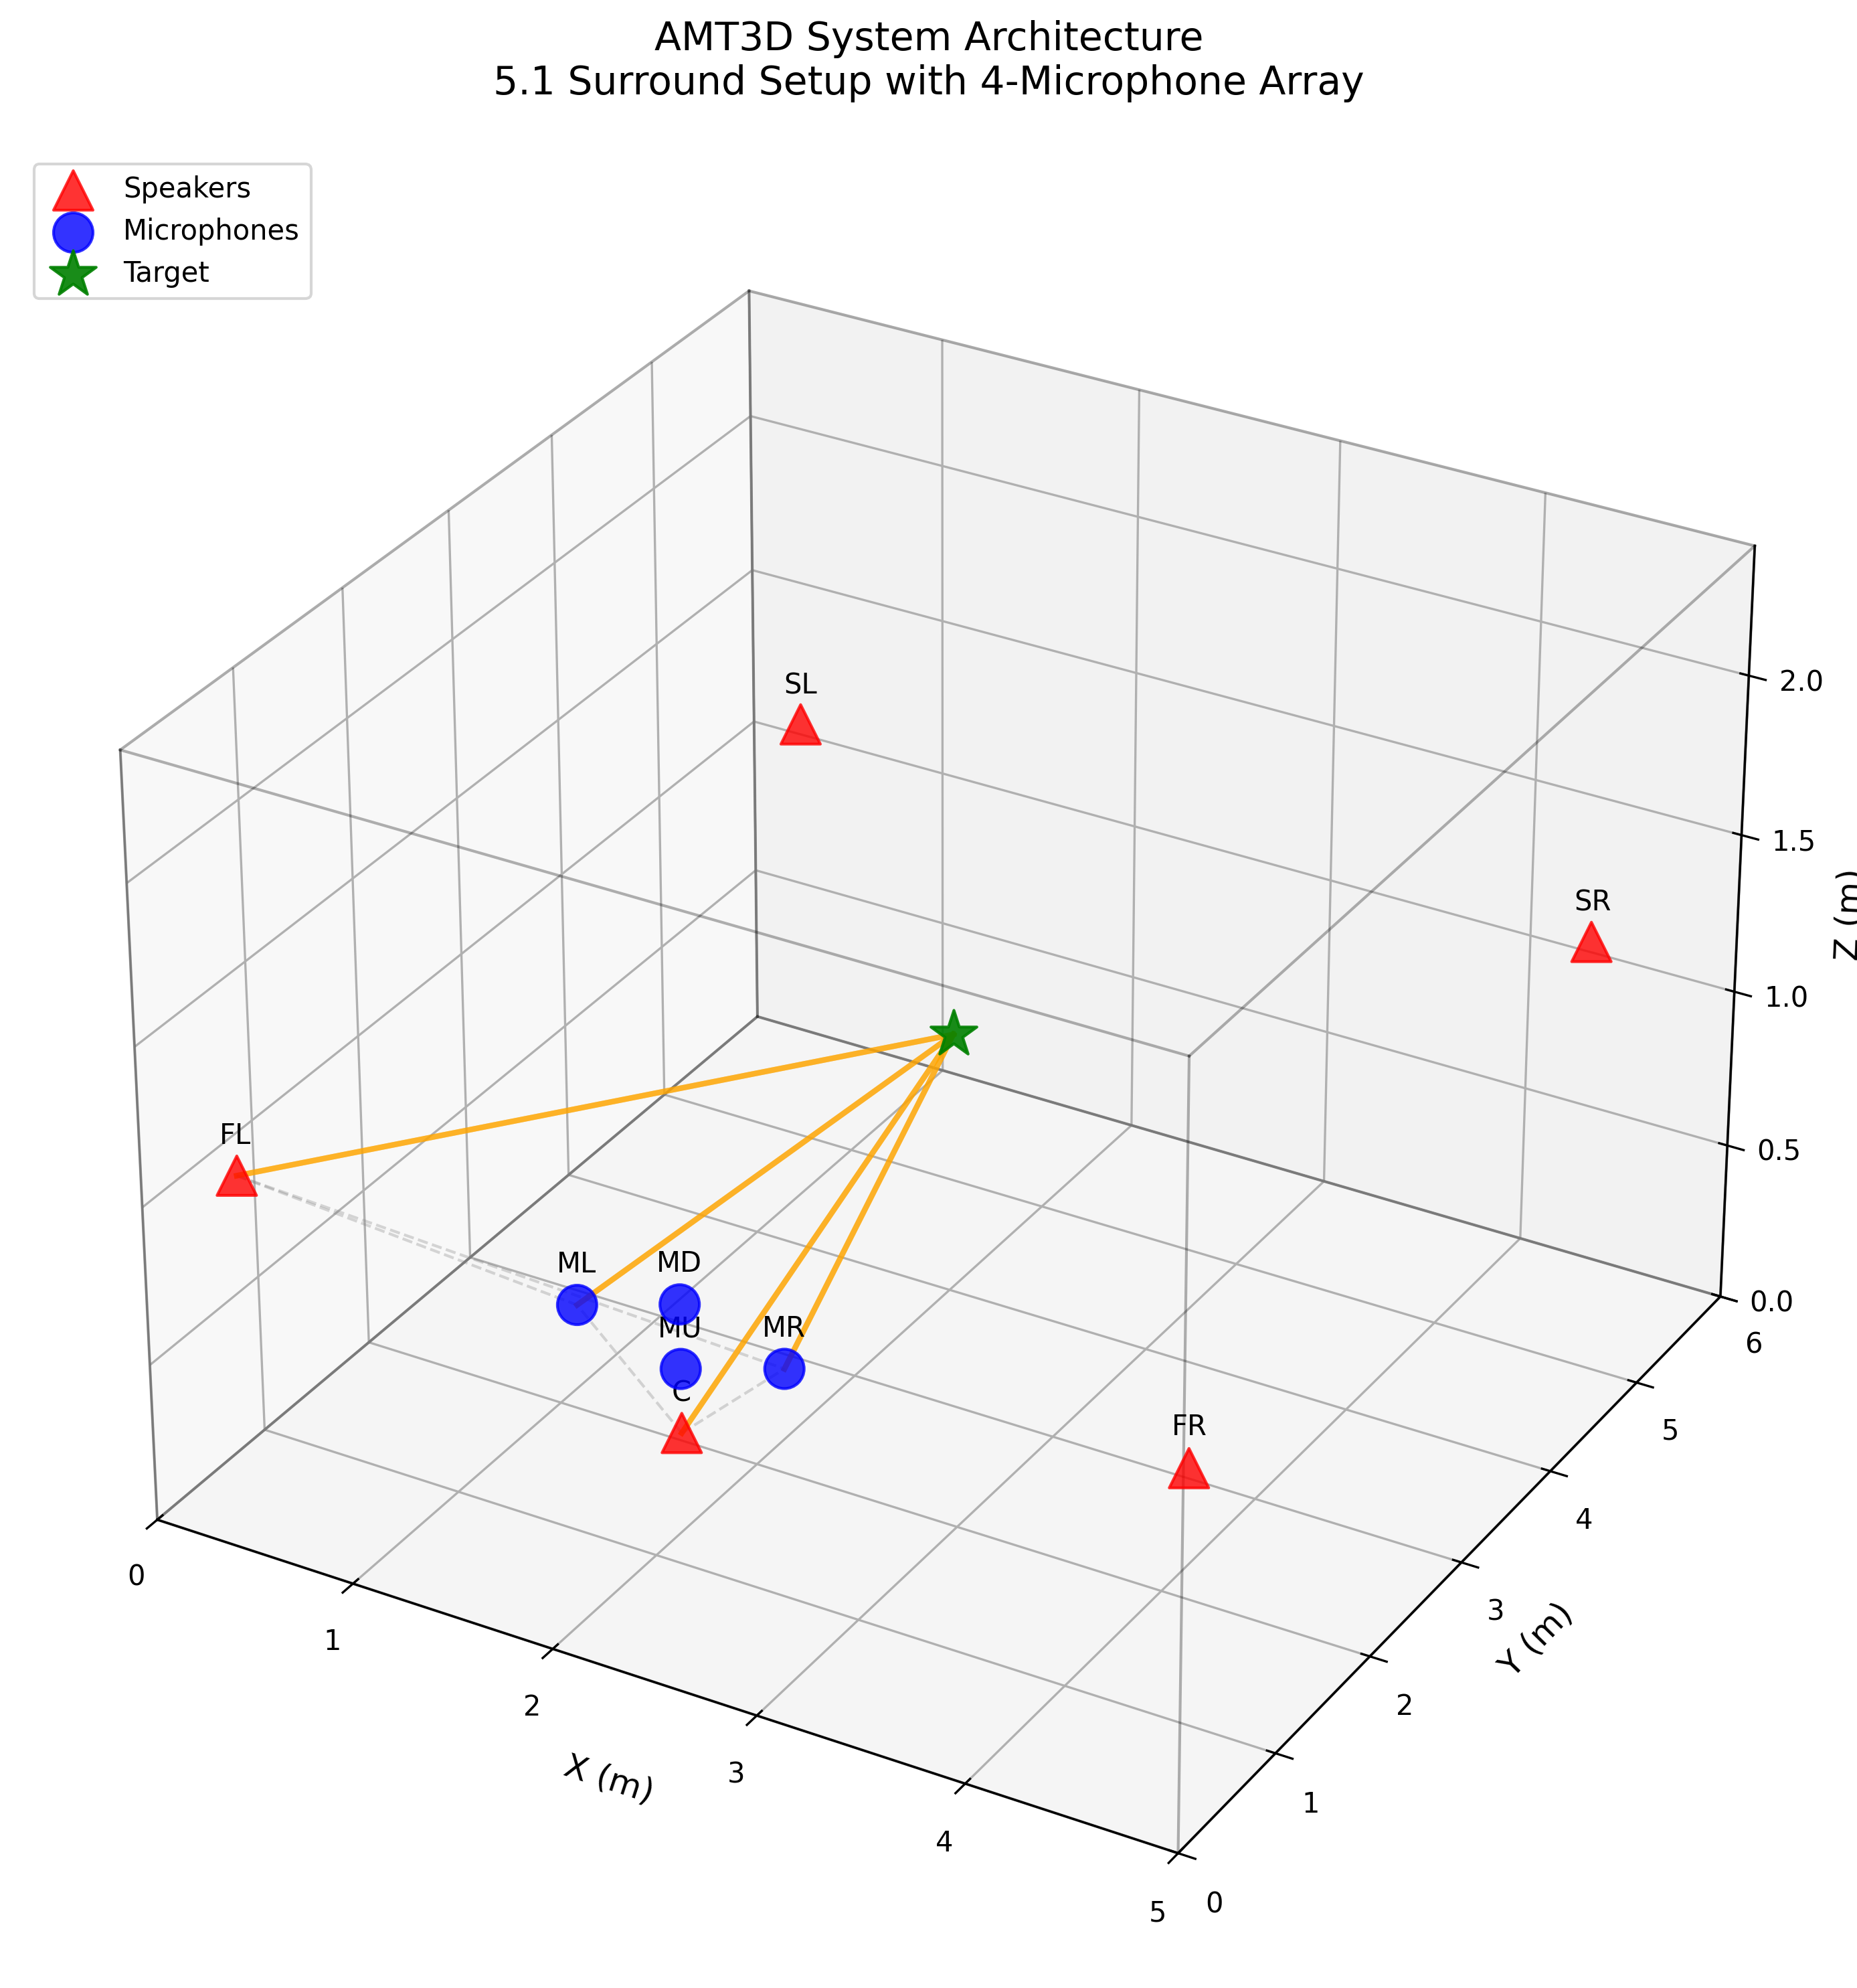
\includegraphics[width=85mm]{final/system_architecture.png}}
\caption{{\it AMT3D system architecture showing the enhanced components for 3D tracking: 9-dimensional state vectors, two-stage multilateration algorithm, adaptive noise handling for z-axis measurements, and temporal continuity constraints. The system builds upon AMT+ foundations while addressing the fundamental challenges of volumetric acoustic tracking.}}
\label{fig:system_architecture}
\end{figure}

\subsection{Fundamental Challenges in 3D Extension}

The transition from 2D to 3D tracking presents several critical challenges:

\begin{itemize}
\item {\em Geometric Ambiguity:} Limited acoustic baseline diversity in the vertical dimension creates geometric degeneracy
\item {\em Computational Complexity:} Multi-ellipsoid intersection problems are significantly more complex than circle intersections
\item {\em Measurement Uncertainty:} Z-axis measurements exhibit higher uncertainty due to typical microphone array geometries
\item {\em State Space Expansion:} Moving from position-only tracking to 9D state vectors increases filter complexity and computational requirements
\item {\em Multipath Effects:} 3D room acoustics introduce more complex reflection patterns
\end{itemize}

\section{Microphone Array Configurations and Challenges}

\subsection{Array Configuration Design Rationale}

To evaluate the 3D extension across different deployment scenarios, we tested three distinct microphone array configurations, each addressing specific geometric constraints and application requirements:

\begin{itemize}
\item {\em Compact 4-Microphone Array:} Designed for space-constrained deployments with balanced 3D coverage
\item {\em Distributed 4-Microphone Array:} Optimized for maximum geometric diversity and triangulation accuracy
\item {\em Soundbar 3-Microphone Array:} Linear arrangement suitable for consumer electronics integration
\end{itemize}

Figure \ref{fig:config_comparison} shows the performance characteristics of these three array configurations, demonstrating the trade-offs between geometric constraints and tracking accuracy.

\begin{figure}[t]
\centerline{
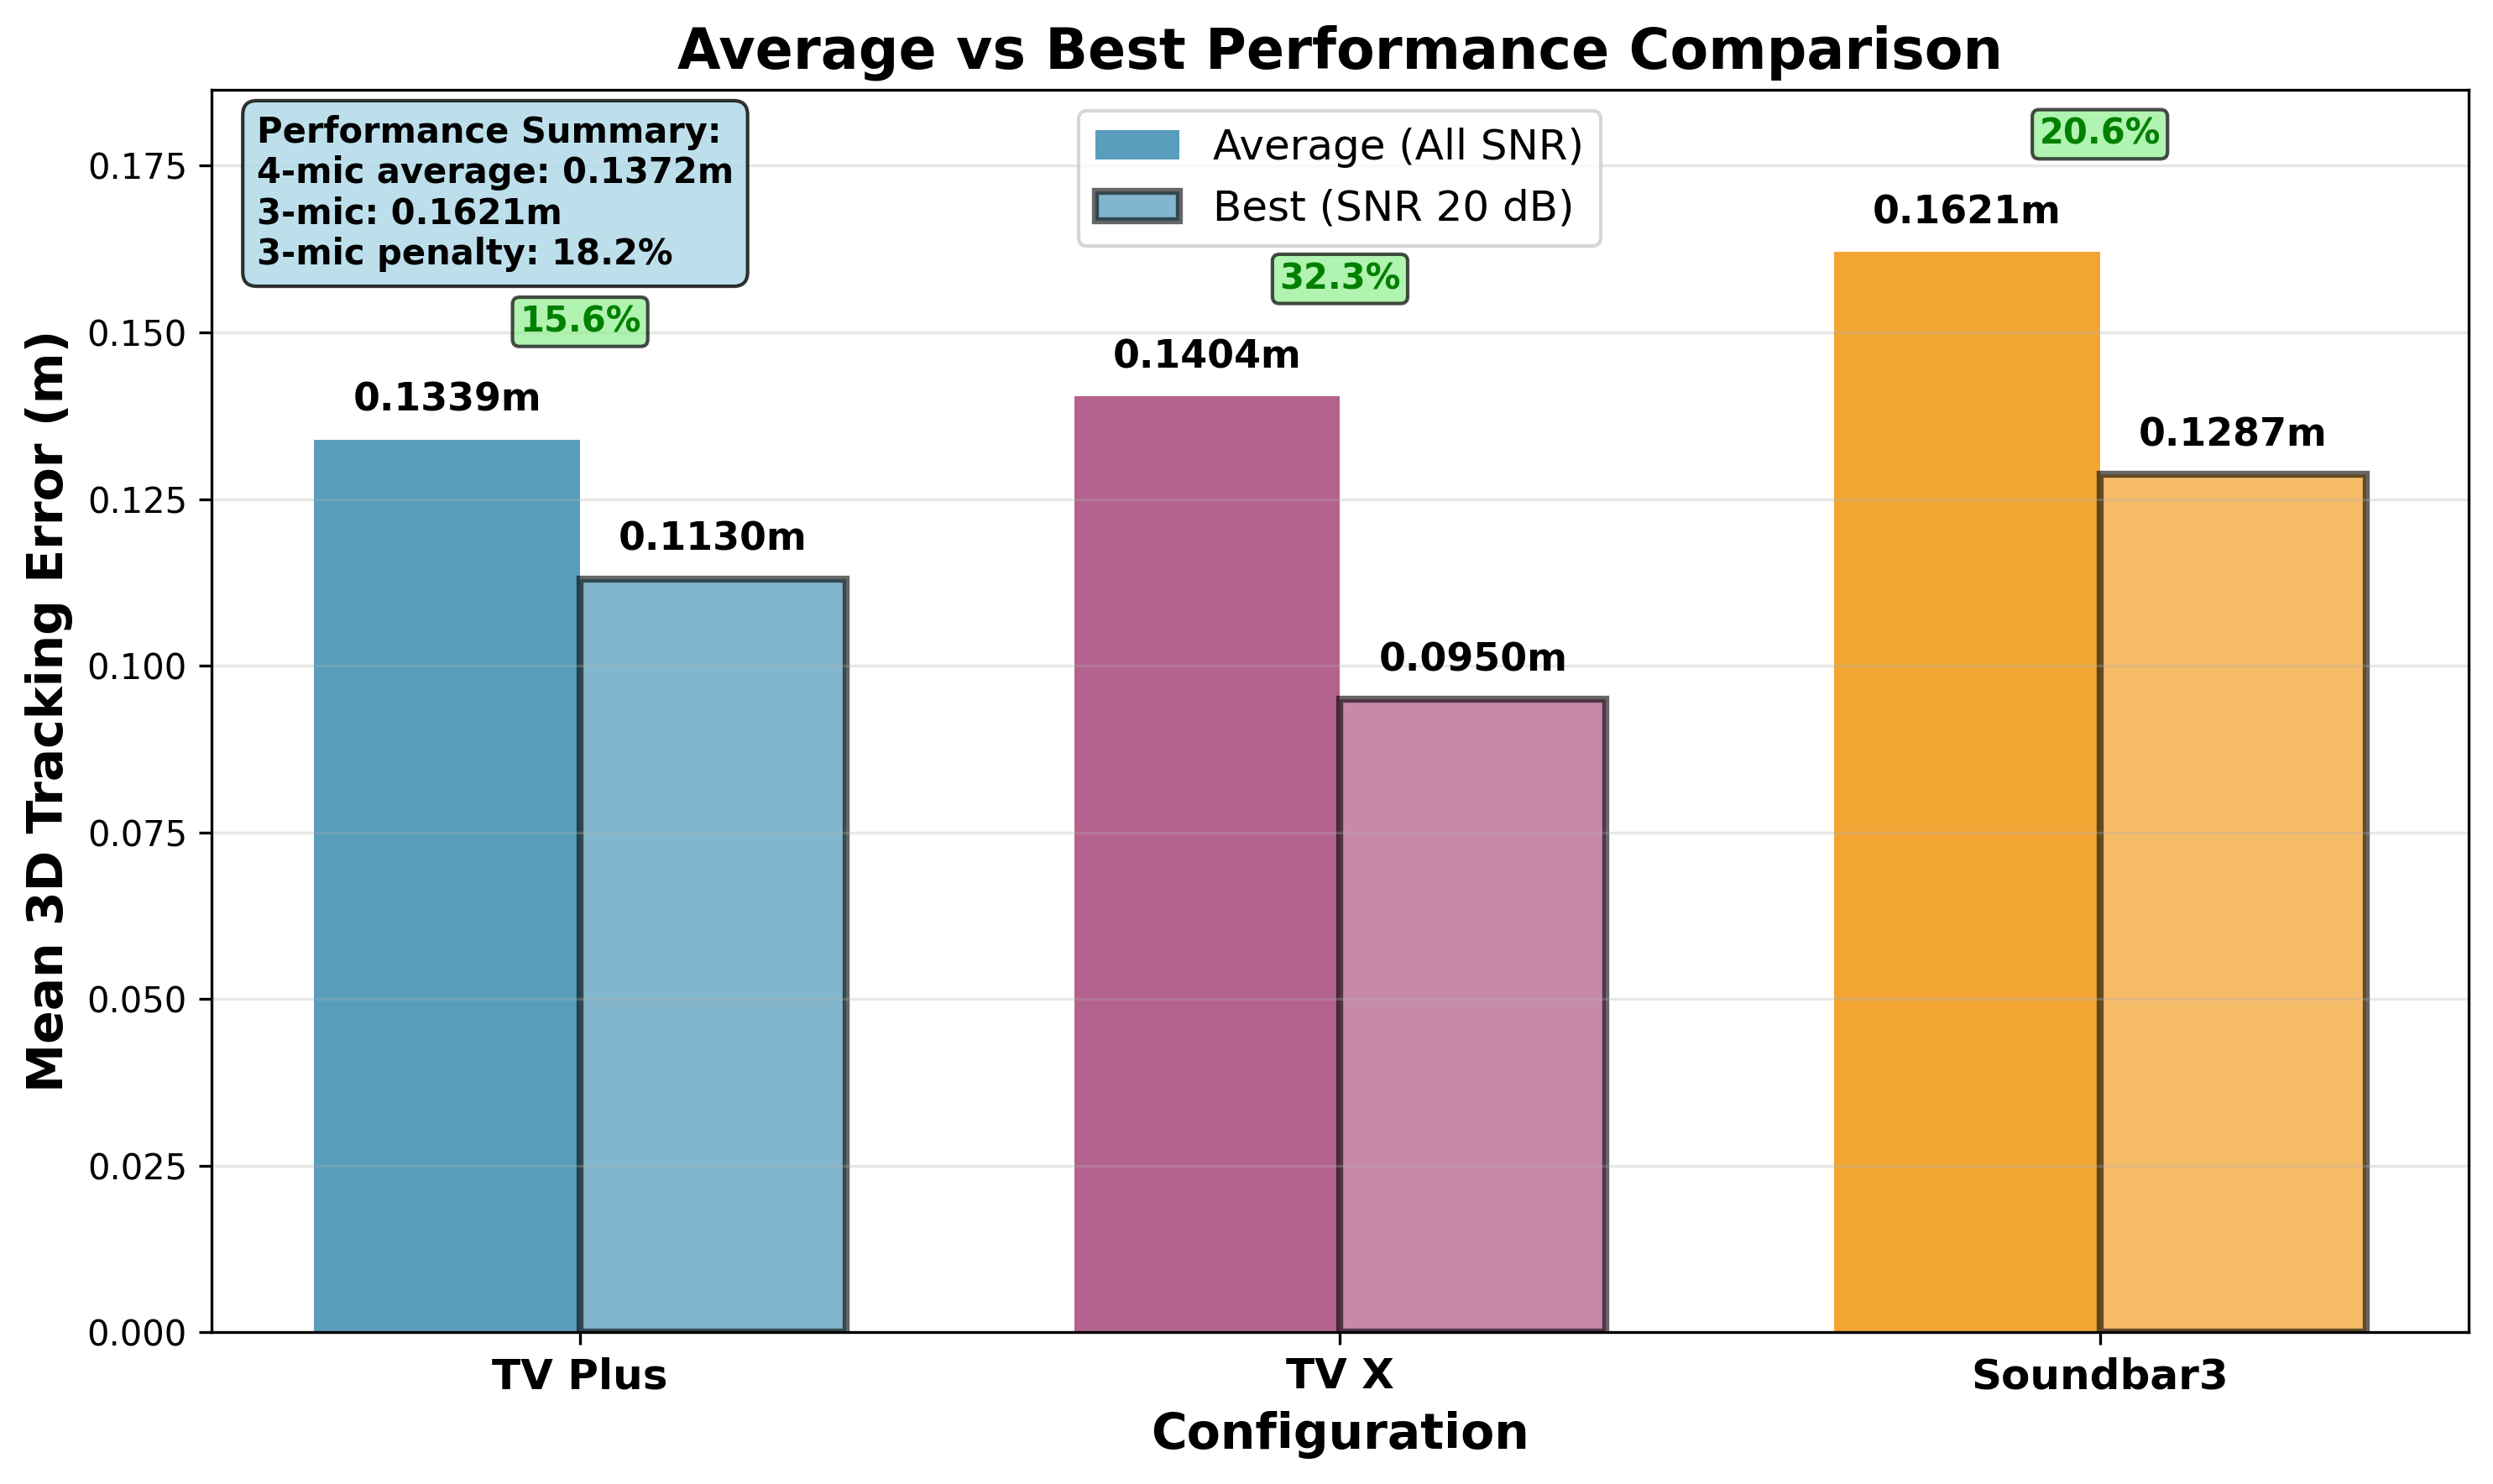
\includegraphics[width=85mm]{final/simple_three_config_performance_comparison.png}}
\caption{{\it Performance comparison of three microphone array configurations showing average and optimal tracking errors. The compact 4-mic array provides consistent performance, the distributed 4-mic array excels in optimal conditions, and the soundbar 3-mic array offers competitive performance with hardware simplification.}}
\label{fig:config_comparison}
\end{figure}

\subsection{Challenge: Geometric Ambiguity in Vertical Dimension}

One of the primary challenges in 3D extension is the limited geometric diversity in the vertical dimension. Even with the home theater setup providing speakers at different heights (0.7m-1.2m) and varied positioning, vertical triangulation remains more constrained than horizontal localization.

{\bf Problem:} Despite the home theater setup providing some vertical diversity, the acoustic baselines for vertical triangulation are still more limited than horizontal baselines, leading to:

\begin{itemize}
\item Reduced precision in z-coordinate estimation
\item Increased sensitivity to measurement noise in vertical direction
\item Geometric degeneracy when targets are directly above/below array center
\end{itemize}

{\bf Solution Approach:} We address this through:

\begin{itemize}
\item {\em Adaptive measurement noise modeling:} Increased uncertainty weights for z-axis measurements
\item {\em Temporal continuity constraints:} Penalize unrealistic vertical movements
\item {\em Multi-array fusion:} When possible, combine measurements from arrays at different heights
\end{itemize}

\section{Technical Implementation and Solutions}

\subsection{Enhanced State Modeling for 3D Tracking}

{\bf Challenge:} The original AMT+ system performs position-only tracking in 2D space using ellipse intersections. Extending to 3D requires not only adding the third spatial dimension but also implementing sophisticated motion modeling to handle the increased complexity and geometric ambiguities.

{\bf Solution:} We implement a 9-dimensional state vector to track position, velocity, and acceleration in all three dimensions, representing a fundamental enhancement from AMT+'s position-only approach:

\begin{equation}
\mathbf{x} = [x, y, z, v_x, v_y, v_z, a_x, a_y, a_z]^T
\label{eq:state_vector}
\end{equation}

The state transition matrix incorporates kinematic equations for constant acceleration motion in 3D:

\begin{equation}
\mathbf{F} = \begin{bmatrix}
\mathbf{I}_3 & \Delta t \mathbf{I}_3 & \frac{1}{2}\Delta t^2 \mathbf{I}_3 \\
\mathbf{0} & \mathbf{I}_3 & \Delta t \mathbf{I}_3 \\
\mathbf{0} & \mathbf{0} & \mathbf{I}_3
\end{bmatrix}
\label{eq:transition_matrix}
\end{equation}

This expansion from position-only tracking to 9D state modeling increases computational complexity but provides the necessary degrees of freedom for full 3D motion modeling and temporal stability that pure geometric intersection approaches cannot achieve.

\subsection{Two-Stage Multi-Ellipsoid Intersection Algorithm}

{\bf Challenge:} The AMT+ 2D system solves ellipse intersection problems in planar space. Extending to 3D requires solving multi-ellipsoid intersection problems, which are significantly more complex both geometrically and computationally, particularly for the vertical dimension where geometric constraints create ambiguities.

{\bf Problem Formulation:} Each speaker-microphone pair contributes an ellipsoid with foci at the speaker and microphone positions. The target localization becomes a multi-ellipsoid intersection optimization problem:

\begin{equation}
\mathbf{p}^* = \arg\min_{\mathbf{p}} \sum_{i=1}^{N} |\|\mathbf{p} - \mathbf{f}_{i1}\| + \|\mathbf{p} - \mathbf{f}_{i2}\| - L_i|^2
\label{eq:ellipsoid_optimization}
\end{equation}

where $\mathbf{f}_{i1}$ and $\mathbf{f}_{i2}$ are the ellipsoid foci (speaker and microphone positions), and $L_i$ is the measured acoustic path length.

Figure \ref{fig:ellipsoid_intersection} demonstrates the ellipsoid intersection process during active tracking.

\begin{figure}[t]
\centerline{
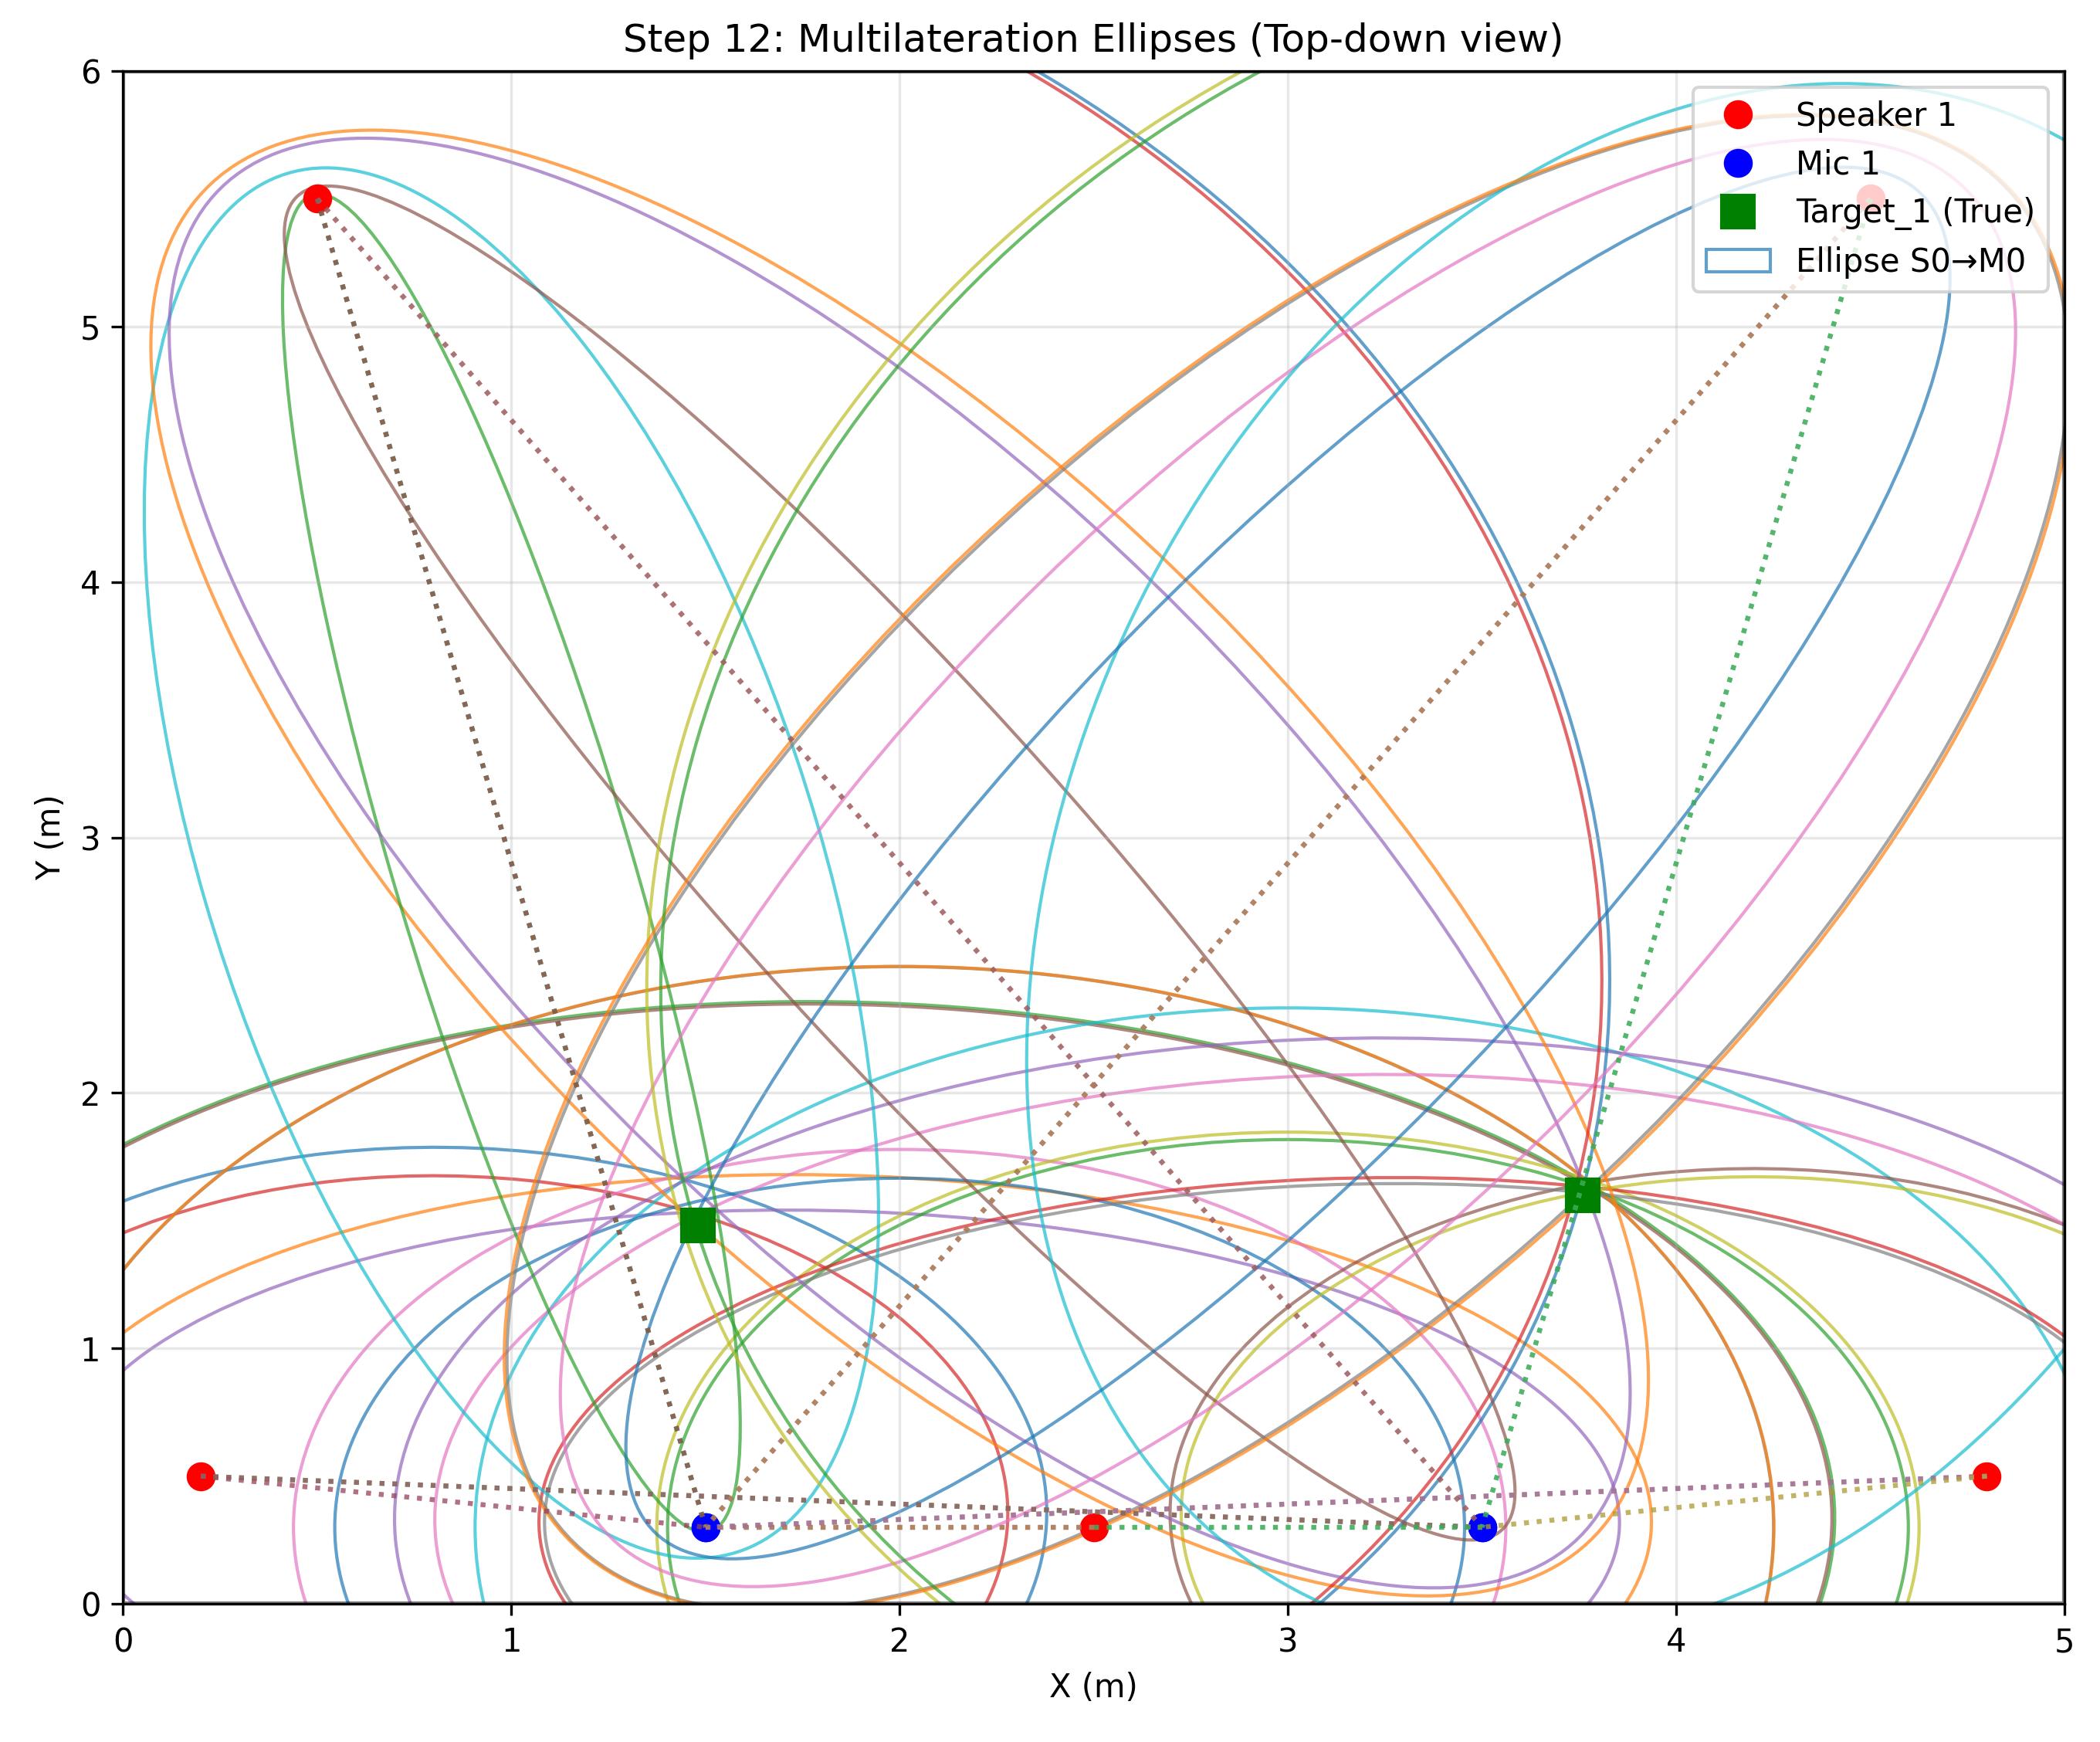
\includegraphics[width=85mm]{final/ellipses_step012.png}}
\caption{{\it Multi-ellipsoid intersection visualization showing acoustic ellipses converging on target position. Each speaker-microphone pair contributes a constraint ellipse, and the target location is determined through two-stage optimization of the intersection problem.}}
\label{fig:ellipsoid_intersection}
\end{figure}

{\bf Two-Stage Solution Implementation:}

We developed a two-stage multilateration algorithm to address the computational complexity and geometric ambiguities inherent in 3D ellipsoid intersection:

{\bf Stage 1: Coarse Grid Search}
\begin{itemize}
\item {\em Adaptive Resolution:} Increased z-axis resolution (2× multiplier) to handle vertical geometric constraints
\item {\em Trajectory-Guided Search:} Uses Kalman filter predictions to focus search around expected positions
\item {\em Ambiguity Detection:} Samples multiple z-levels to detect vertical positioning ambiguities
\item {\em Search Space:} Covers entire room volume with coarse resolution (typically 20×20×40 grid)
\end{itemize}

{\bf Stage 2: Fine Localized Search}
\begin{itemize}
\item {\em Adaptive Resolution Enhancement:} Increases resolution by 50\% when ambiguities are detected
\item {\em Localized Search Region:} Concentrates on area around coarse-stage optimum
\item {\em Z-Axis Enhancement:} Doubles z-resolution and expands z-search range for ambiguous cases
\item {\em Trajectory Consistency:} Validates results against motion model predictions
\end{itemize}

{\bf Continuity Constraints:}

To address z-axis instability discovered during implementation, we incorporate temporal continuity constraints:

\begin{equation}
E_{total} = E_{ellipsoid} + \alpha_z (z_t - z_{t-1})^2
\label{eq:continuity_constraint}
\end{equation}

where $\alpha_z = 0.5$ penalizes sudden vertical movements while preserving legitimate motion patterns.

\subsection{Adaptive Noise Handling for Vertical Measurements}

{\bf Challenge:} During implementation, we discovered that z-axis measurements are inherently less stable than horizontal measurements due to typical microphone array geometries.

{\bf Problem Identified:} Standard noise models assume isotropic measurement uncertainty. However, our experiments revealed that vertical position estimates exhibit higher variance and instability.

{\bf Solution:} We implement adaptive measurement noise covariance that accounts for geometric constraints:

\begin{equation}
\mathbf{R} = \text{diag}([r_x, r_y, r_z])
\label{eq:measurement_noise}
\end{equation}

where $r_z > r_x, r_y$ to reflect the increased uncertainty in vertical measurements.

Additionally, we introduce temporal continuity constraints to prevent unrealistic vertical position jumps, as incorporated into the total error function shown in Equation \ref{eq:continuity_constraint}.

\subsection{3D Room Acoustic Modeling}

{\bf Challenge:} 3D environments introduce more complex multipath propagation patterns compared to 2D scenarios.

{\bf Implementation:} We utilize pyroomacoustics \cite{pyroomacoustics} for realistic 3D acoustic simulation including:

\begin{itemize}
\item 3D reflection pattern modeling
\item Wall and ceiling absorption effects
\item Realistic propagation delays in 3D space
\item Enhanced multipath separation algorithms
\end{itemize}


\section{Performance Evaluation and Results}

\subsection{Evaluation Methodology}

We evaluated the 3D extension performance across different noise conditions (SNR 0, 5, 10, 20 dB) and microphone array configurations to understand the system's behavior across various operational scenarios.

\subsection{Noise Impact on 3D Tracking Performance}

Figure \ref{fig:snr_analysis} demonstrates how acoustic noise affects both mean and maximum 3D tracking errors across the tested SNR range.

\begin{figure}[t]
\centerline{
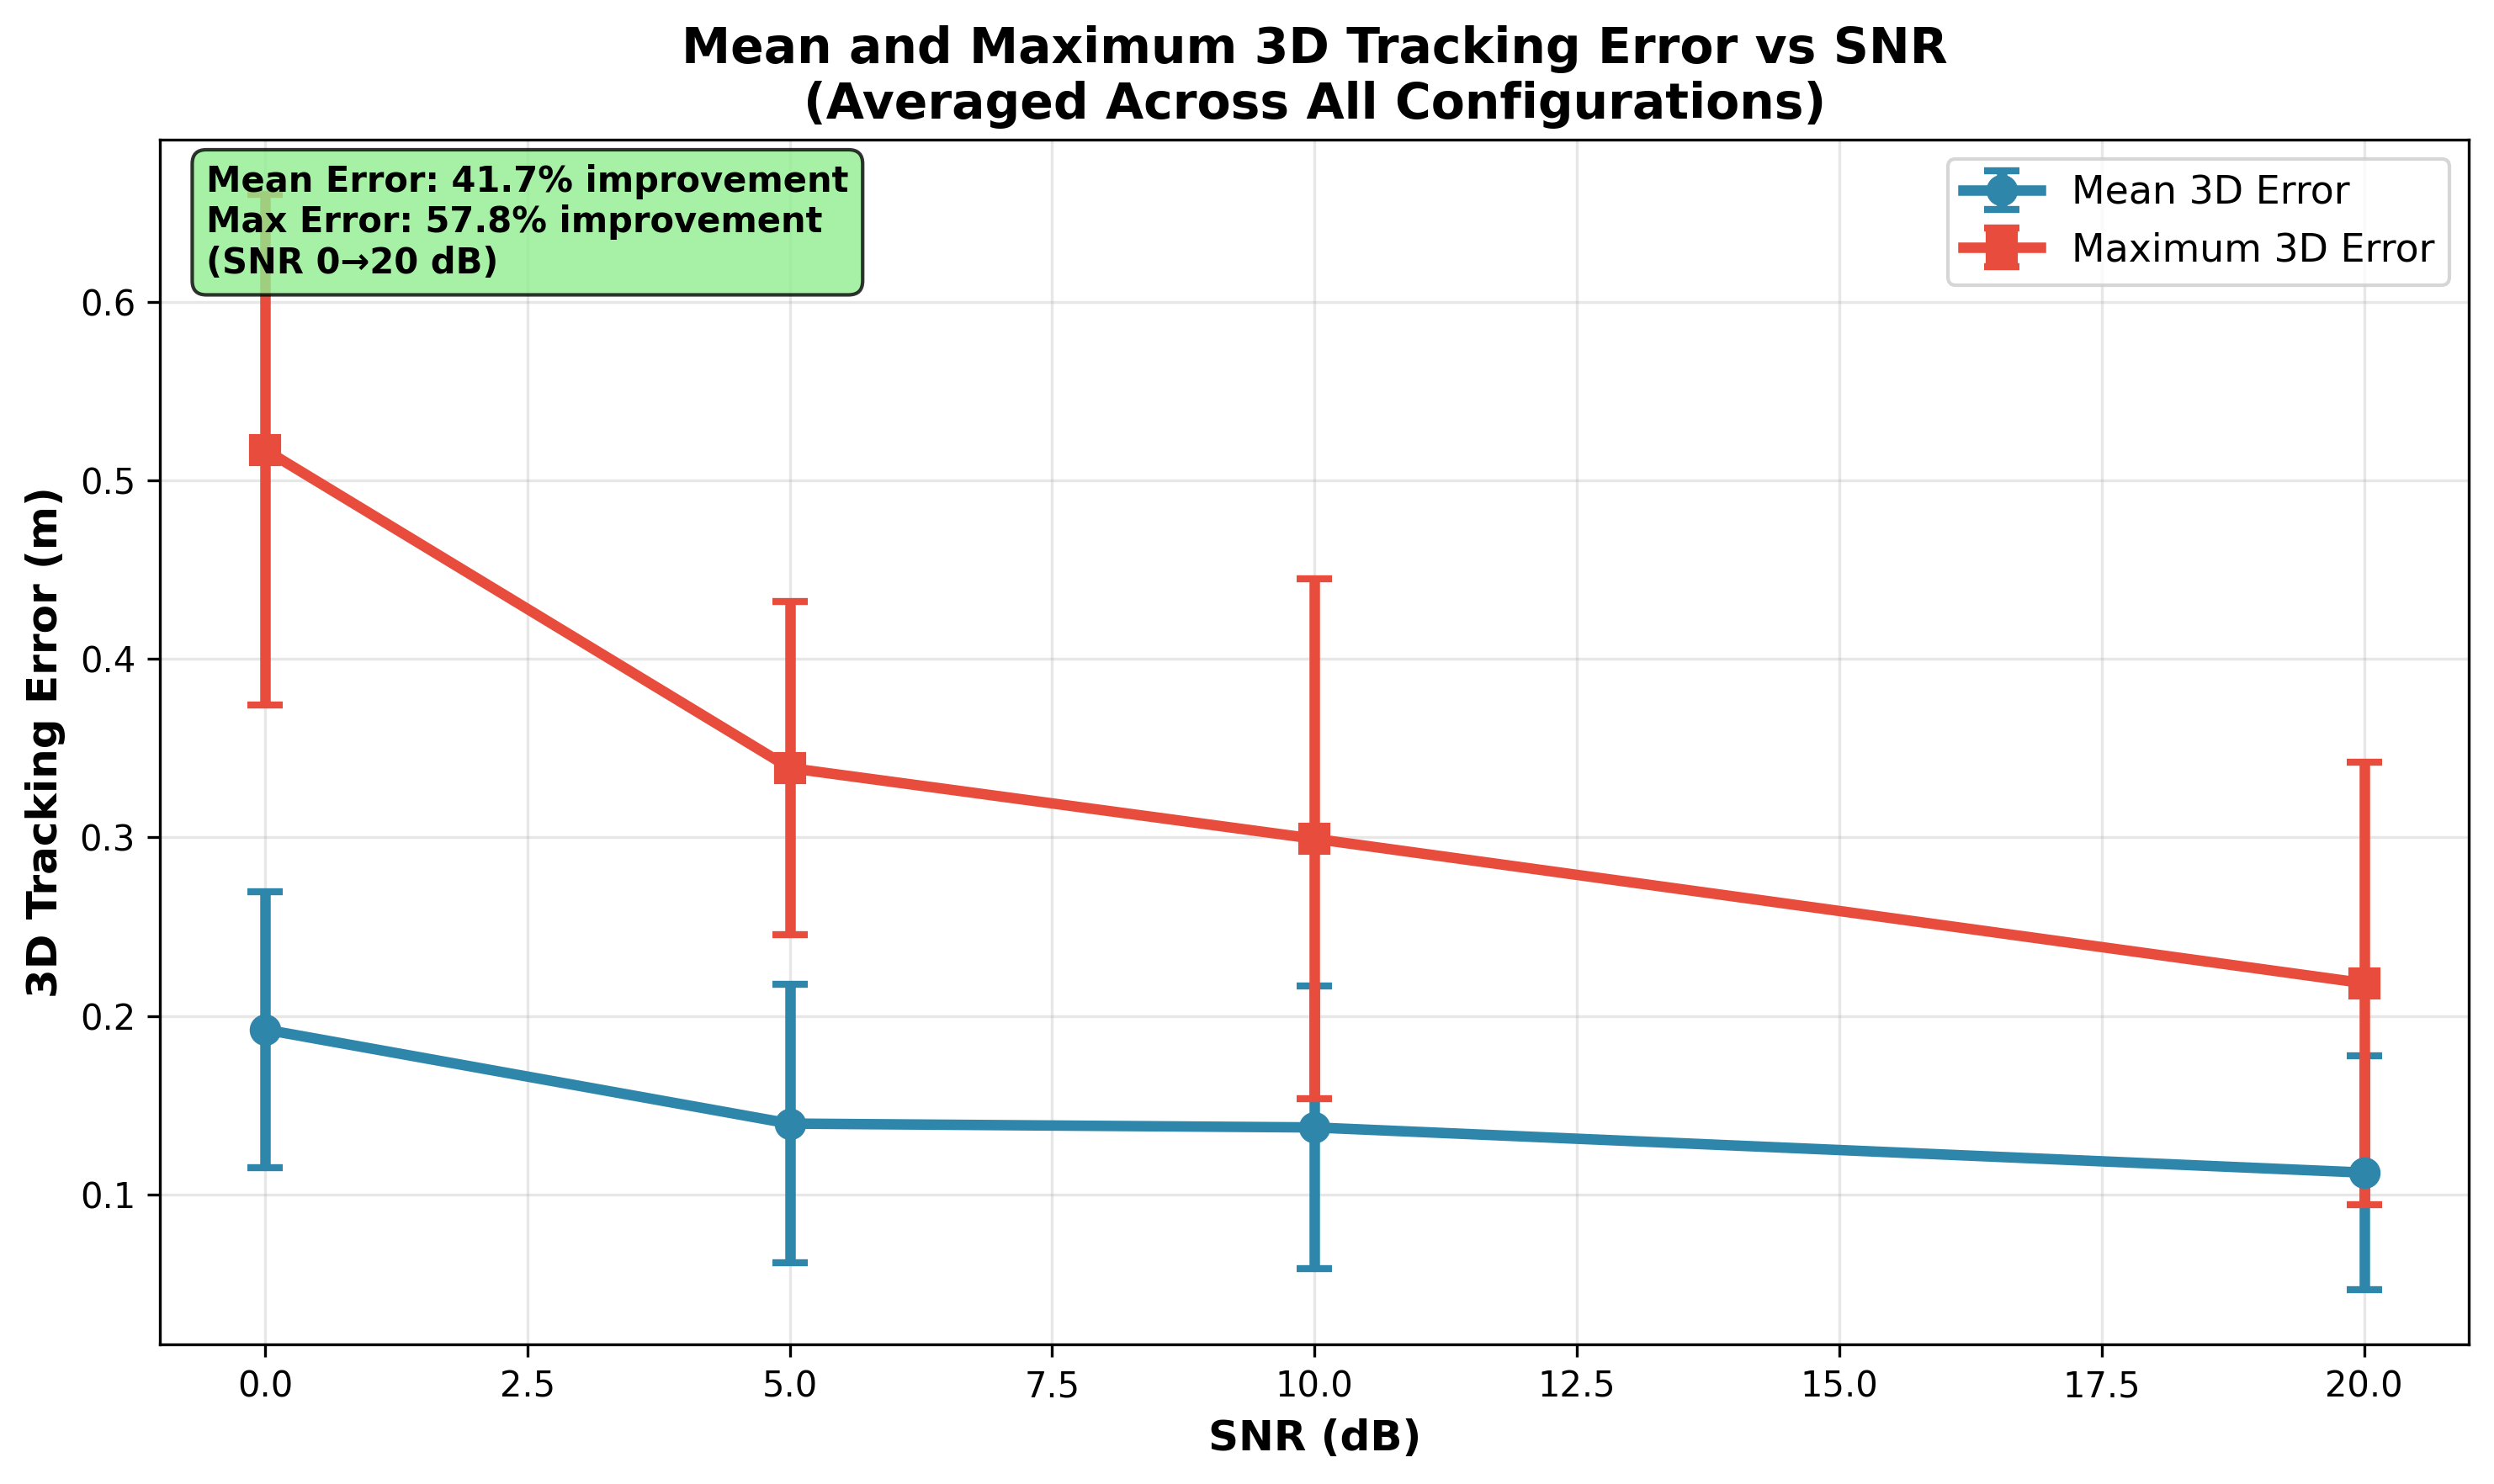
\includegraphics[width=85mm]{final/snr_vs_error_focused.png}}
\caption{{\it Mean and maximum 3D tracking error versus SNR levels, averaged across all three microphone configurations. The results show that mean errors decrease from 0.192 m at SNR 0 dB to 0.112 m at SNR 20 dB (41.7\% improvement), while maximum errors decrease from approximately 0.54 m to 0.20 m (62.9\% improvement), demonstrating the system's robustness across diverse acoustic conditions.}}
\label{fig:snr_analysis}
\end{figure}

The results reveal several important characteristics of 3D acoustic tracking under noise:

\begin{itemize}
\item {\em Consistent Improvement Pattern:} Both mean and maximum errors decrease monotonically with increasing SNR, indicating stable algorithm behavior
\item {\em Maximum Error Sensitivity:} Maximum errors show greater sensitivity to noise (62.9\% improvement) than mean errors (41.7\% improvement), suggesting that extreme outliers are more affected by acoustic interference
\item {\em Practical Performance Range:} Even under challenging conditions (SNR 0 dB), mean tracking errors remain below 0.2 m, demonstrating practical feasibility
\item {\em Error Bounds:} The gap between mean and maximum errors indicates the system's reliability, with maximum errors approximately 2.5-3× the mean errors across all SNR levels
\end{itemize}

\subsection{Error Distribution and Statistical Analysis}

Figure \ref{fig:error_metrics} provides detailed analysis of different error metrics across noise conditions, revealing the statistical characteristics of 3D tracking performance.

\begin{figure}[t]
\centerline{
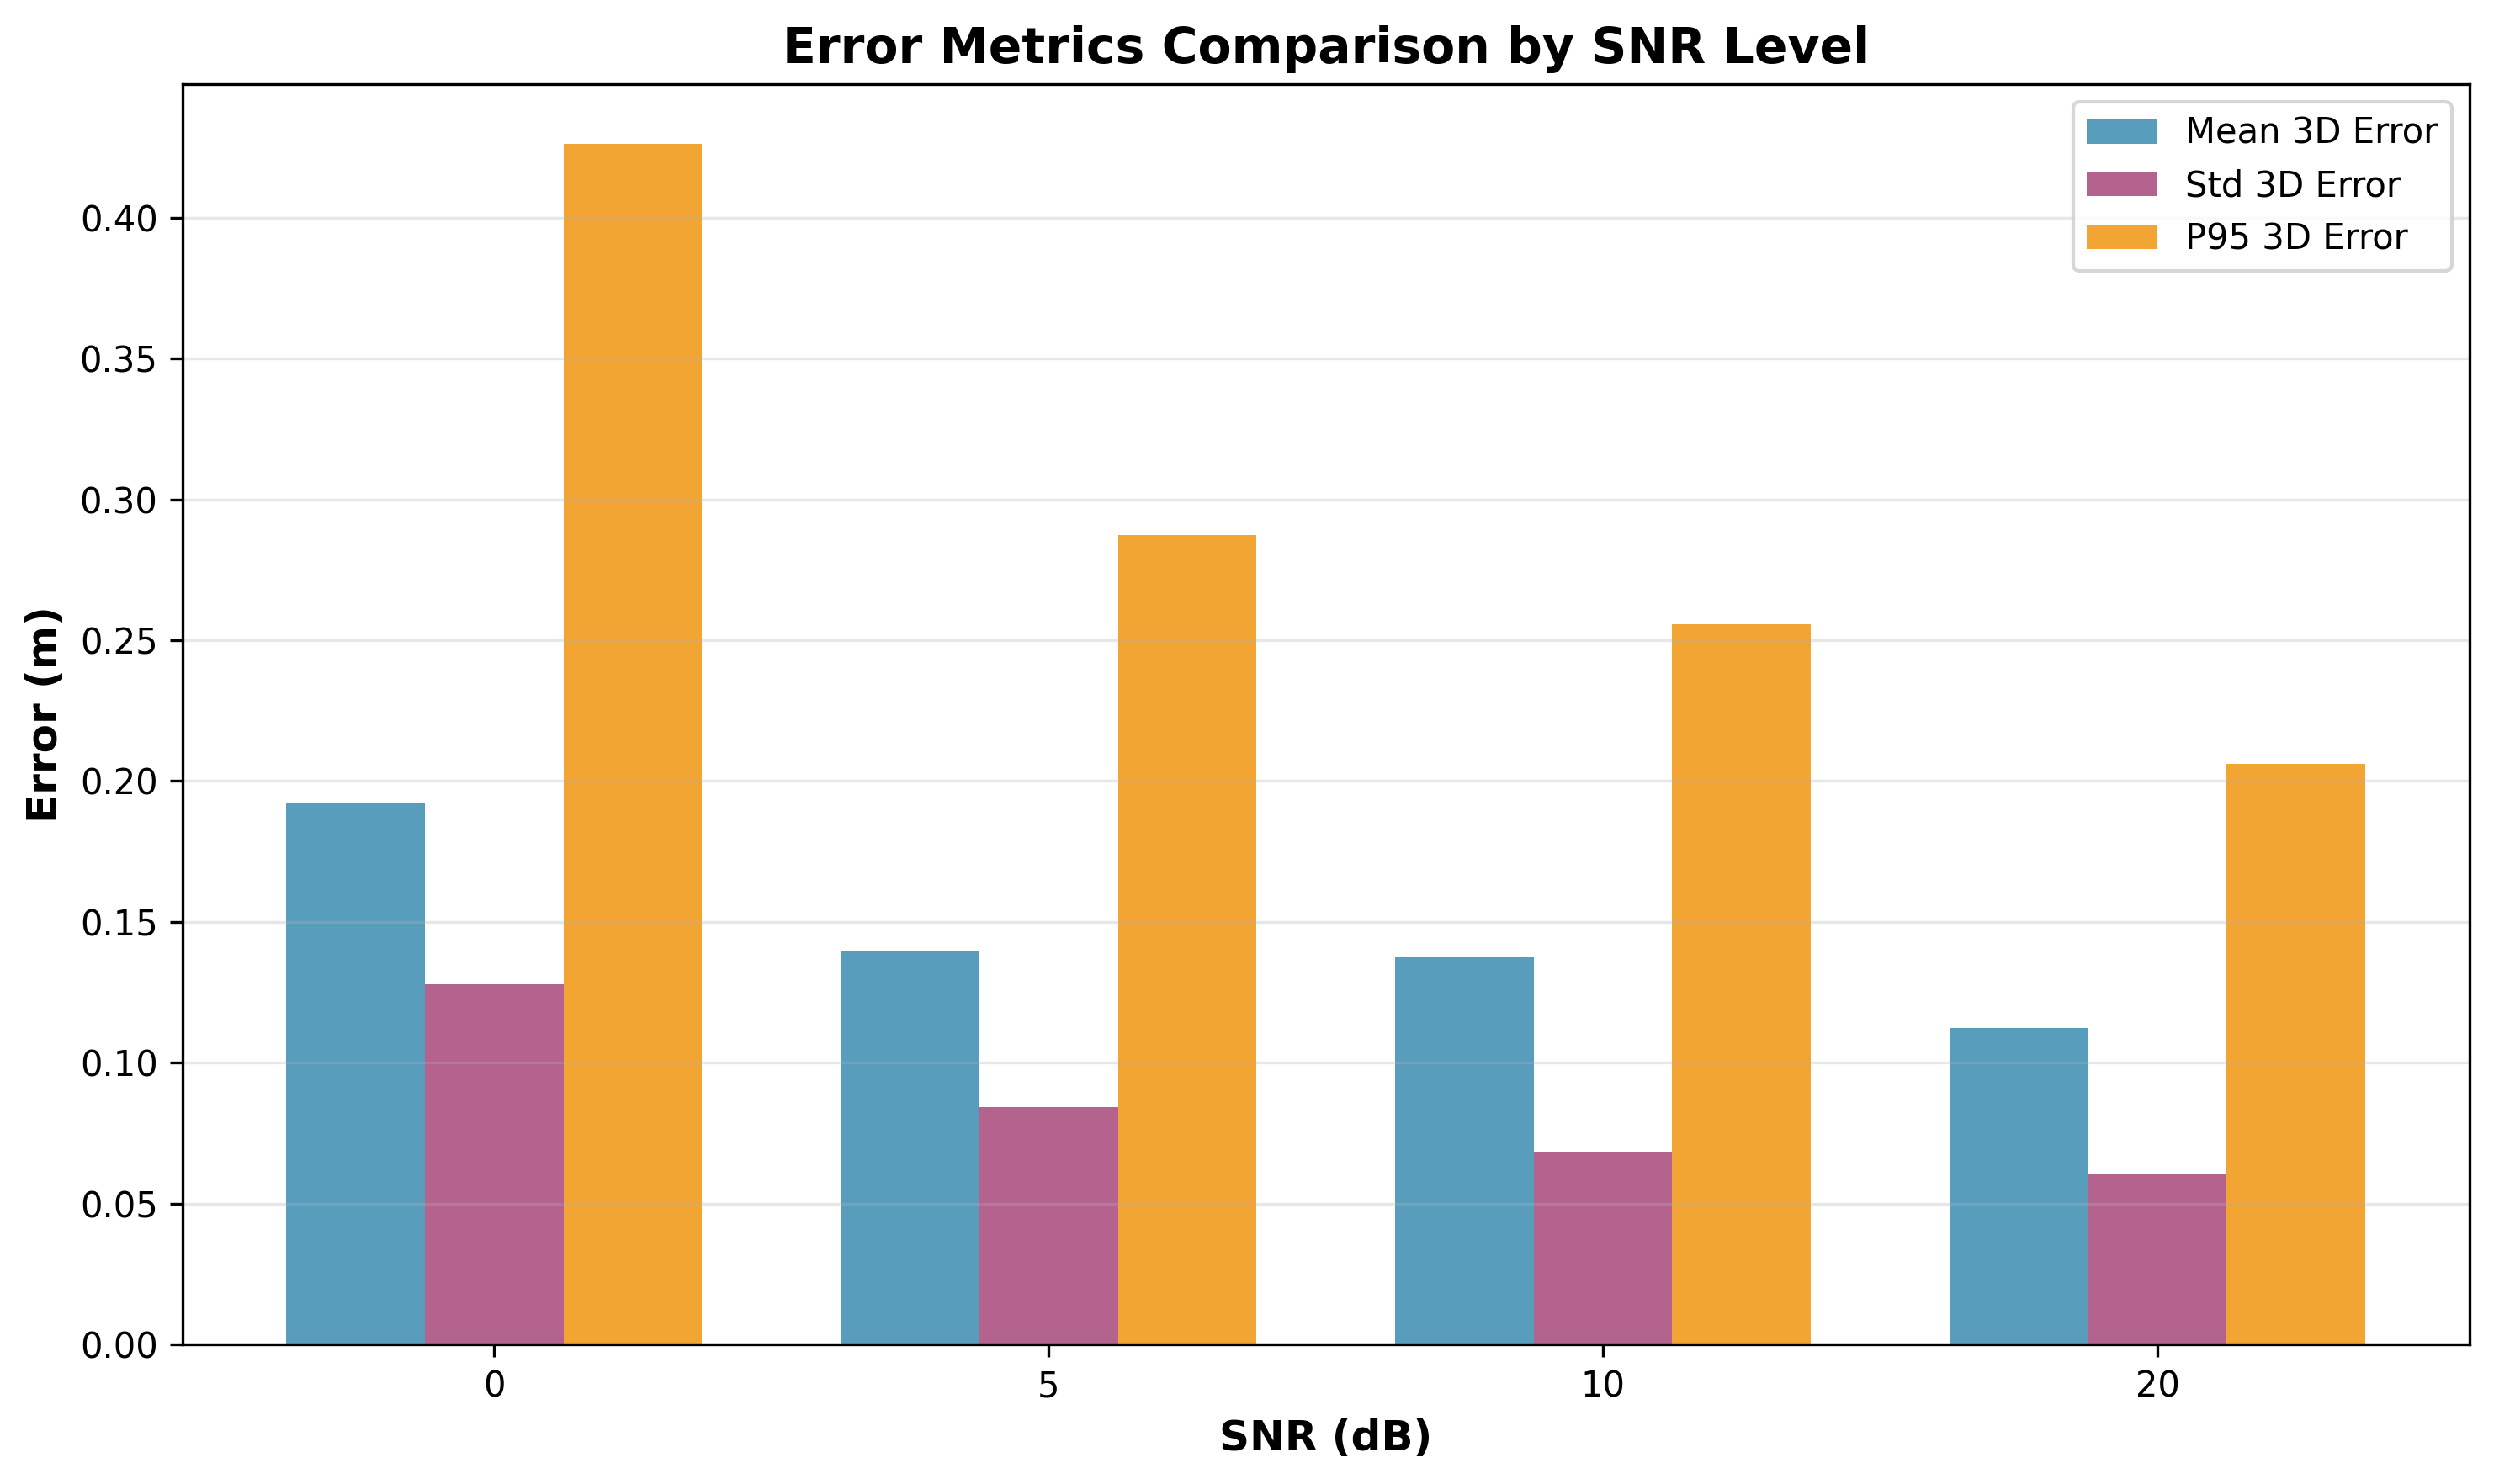
\includegraphics[width=85mm]{final/error_metrics_comparison.png}}
\caption{{\it Error metrics comparison showing mean 3D error, standard deviation, and 95th percentile tracking errors across SNR levels from 0 to 20 dB. All three metrics follow similar improvement patterns: mean errors decrease from 0.192 m to 0.112 m, standard deviations reduce from 0.14 m to 0.06 m, and P95 errors improve from 0.44 m to 0.19 m, indicating consistent algorithm behavior across the complete error distribution.}}
\label{fig:error_metrics}
\end{figure}

The statistical analysis reveals important insights about error distribution characteristics:

\begin{itemize}
\item {\em Proportional Error Reduction:} All error metrics (mean, standard deviation, P95) improve proportionally with increasing SNR, maintaining consistent relative relationships across noise conditions
\item {\em Standard Deviation Analysis:} Error standard deviation decreases from 0.14 m to 0.06 m (57\% improvement), indicating that noise not only affects average performance but significantly impacts tracking consistency
\item {\em P95 Performance:} 95th percentile errors range from 0.19 m to 0.44 m, showing that even worst-case scenarios remain within practical bounds for most applications
\item {\em Distribution Stability:} The parallel improvement patterns across all metrics suggest that the underlying error distribution shape remains stable, indicating robust algorithm design
\end{itemize}

\subsection{Temporal Tracking Stability and Consistency}

A critical aspect of 3D tracking is maintaining stability over extended time periods. Figure \ref{fig:temporal_tracking} demonstrates how tracking errors evolve over time for different noise conditions using real trajectory data.

\begin{figure}[t]
\centerline{
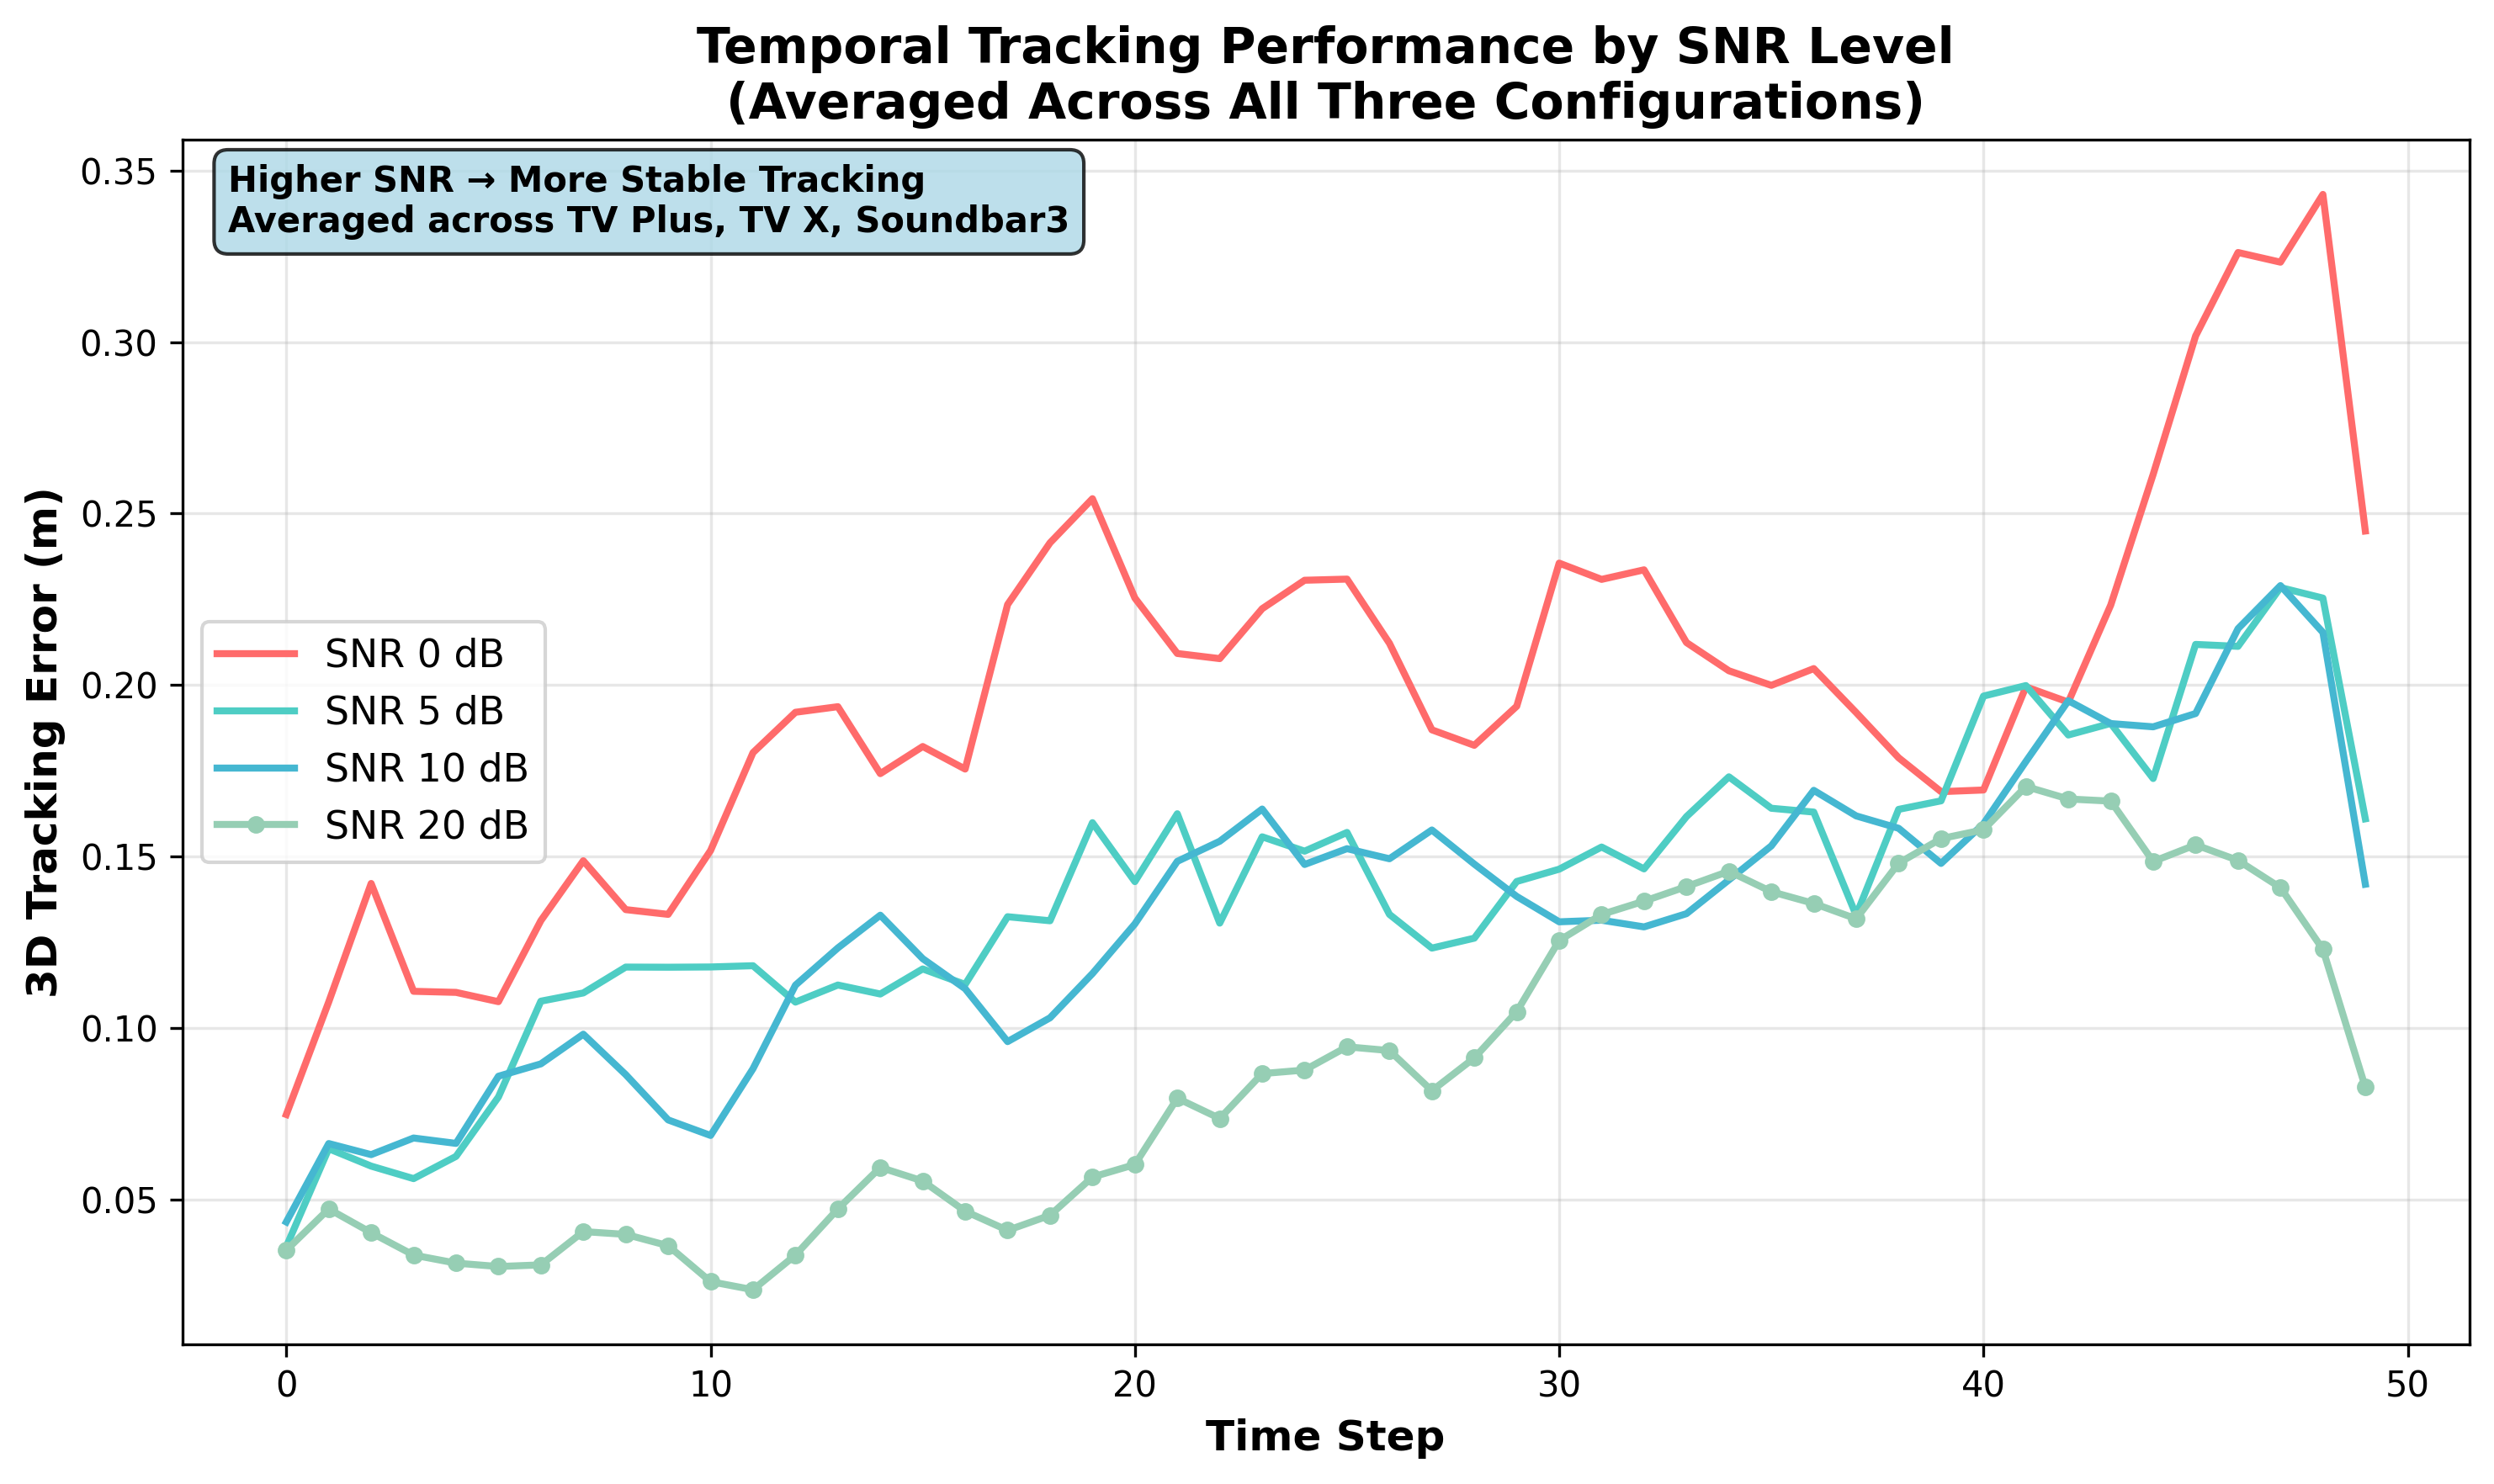
\includegraphics[width=85mm]{final/temporal_tracking_performance.png}}
\caption{{\it Temporal tracking performance showing 3D error evolution over 50 time steps (5 seconds) for different SNR levels, averaged across all three microphone configurations. SNR 0 dB shows high variability (0.05-0.40 m range) with frequent error spikes, while SNR 20 dB demonstrates stable tracking (0.05-0.25 m range) with consistent low-variance performance, validating the effectiveness of temporal continuity constraints.}}
\label{fig:temporal_tracking}
\end{figure}

The temporal analysis reveals critical insights about tracking consistency and stability:

\begin{itemize}
\item {\em Noise-Dependent Variance:} At SNR 0 dB, tracking errors exhibit high temporal variance (0.05-0.40 m range) with frequent error spikes, while SNR 20 dB maintains low variance (0.05-0.25 m range) throughout the tracking sequence
\item {\em Stability Convergence:} Higher SNR conditions (10-20 dB) show convergent behavior where initial tracking uncertainties settle into stable patterns within the first 10-15 time steps
\item {\em Error Spike Patterns:} Low SNR conditions exhibit periodic error spikes that correlate with challenging acoustic conditions, but the system demonstrates recovery capability through temporal continuity constraints
\item {\em Tracking Persistence:} Even under worst-case conditions (SNR 0 dB), the system maintains tracking without complete failure, demonstrating the robustness of the two-stage multilateration approach
\item {\em Continuity Validation:} The smoother temporal profiles at higher SNR levels validate the effectiveness of the temporal continuity constraints (Equation \ref{eq:continuity_constraint}) in preventing unrealistic position jumps
\end{itemize}

\subsection{Performance Results Summary}

The 3D extension achieves the following performance characteristics:

\begin{itemize}
\item {\em Mean tracking errors:} 0.095 m to 0.192 m depending on conditions
\item {\em Array configuration impact:} 4-microphone arrays outperform 3-microphone setup by approximately 18.2\%
\item {\em Noise sensitivity:} Performance degrades gracefully with increasing noise levels
\item {\em Temporal stability:} Consistent tracking maintained over 50-step sequences
\end{itemize}

\section{Trajectory Visualization and Validation}

Figure \ref{fig:trajectories} shows example trajectory tracking results demonstrating the system's 3D tracking capabilities.

\begin{figure}[t]
\centerline{
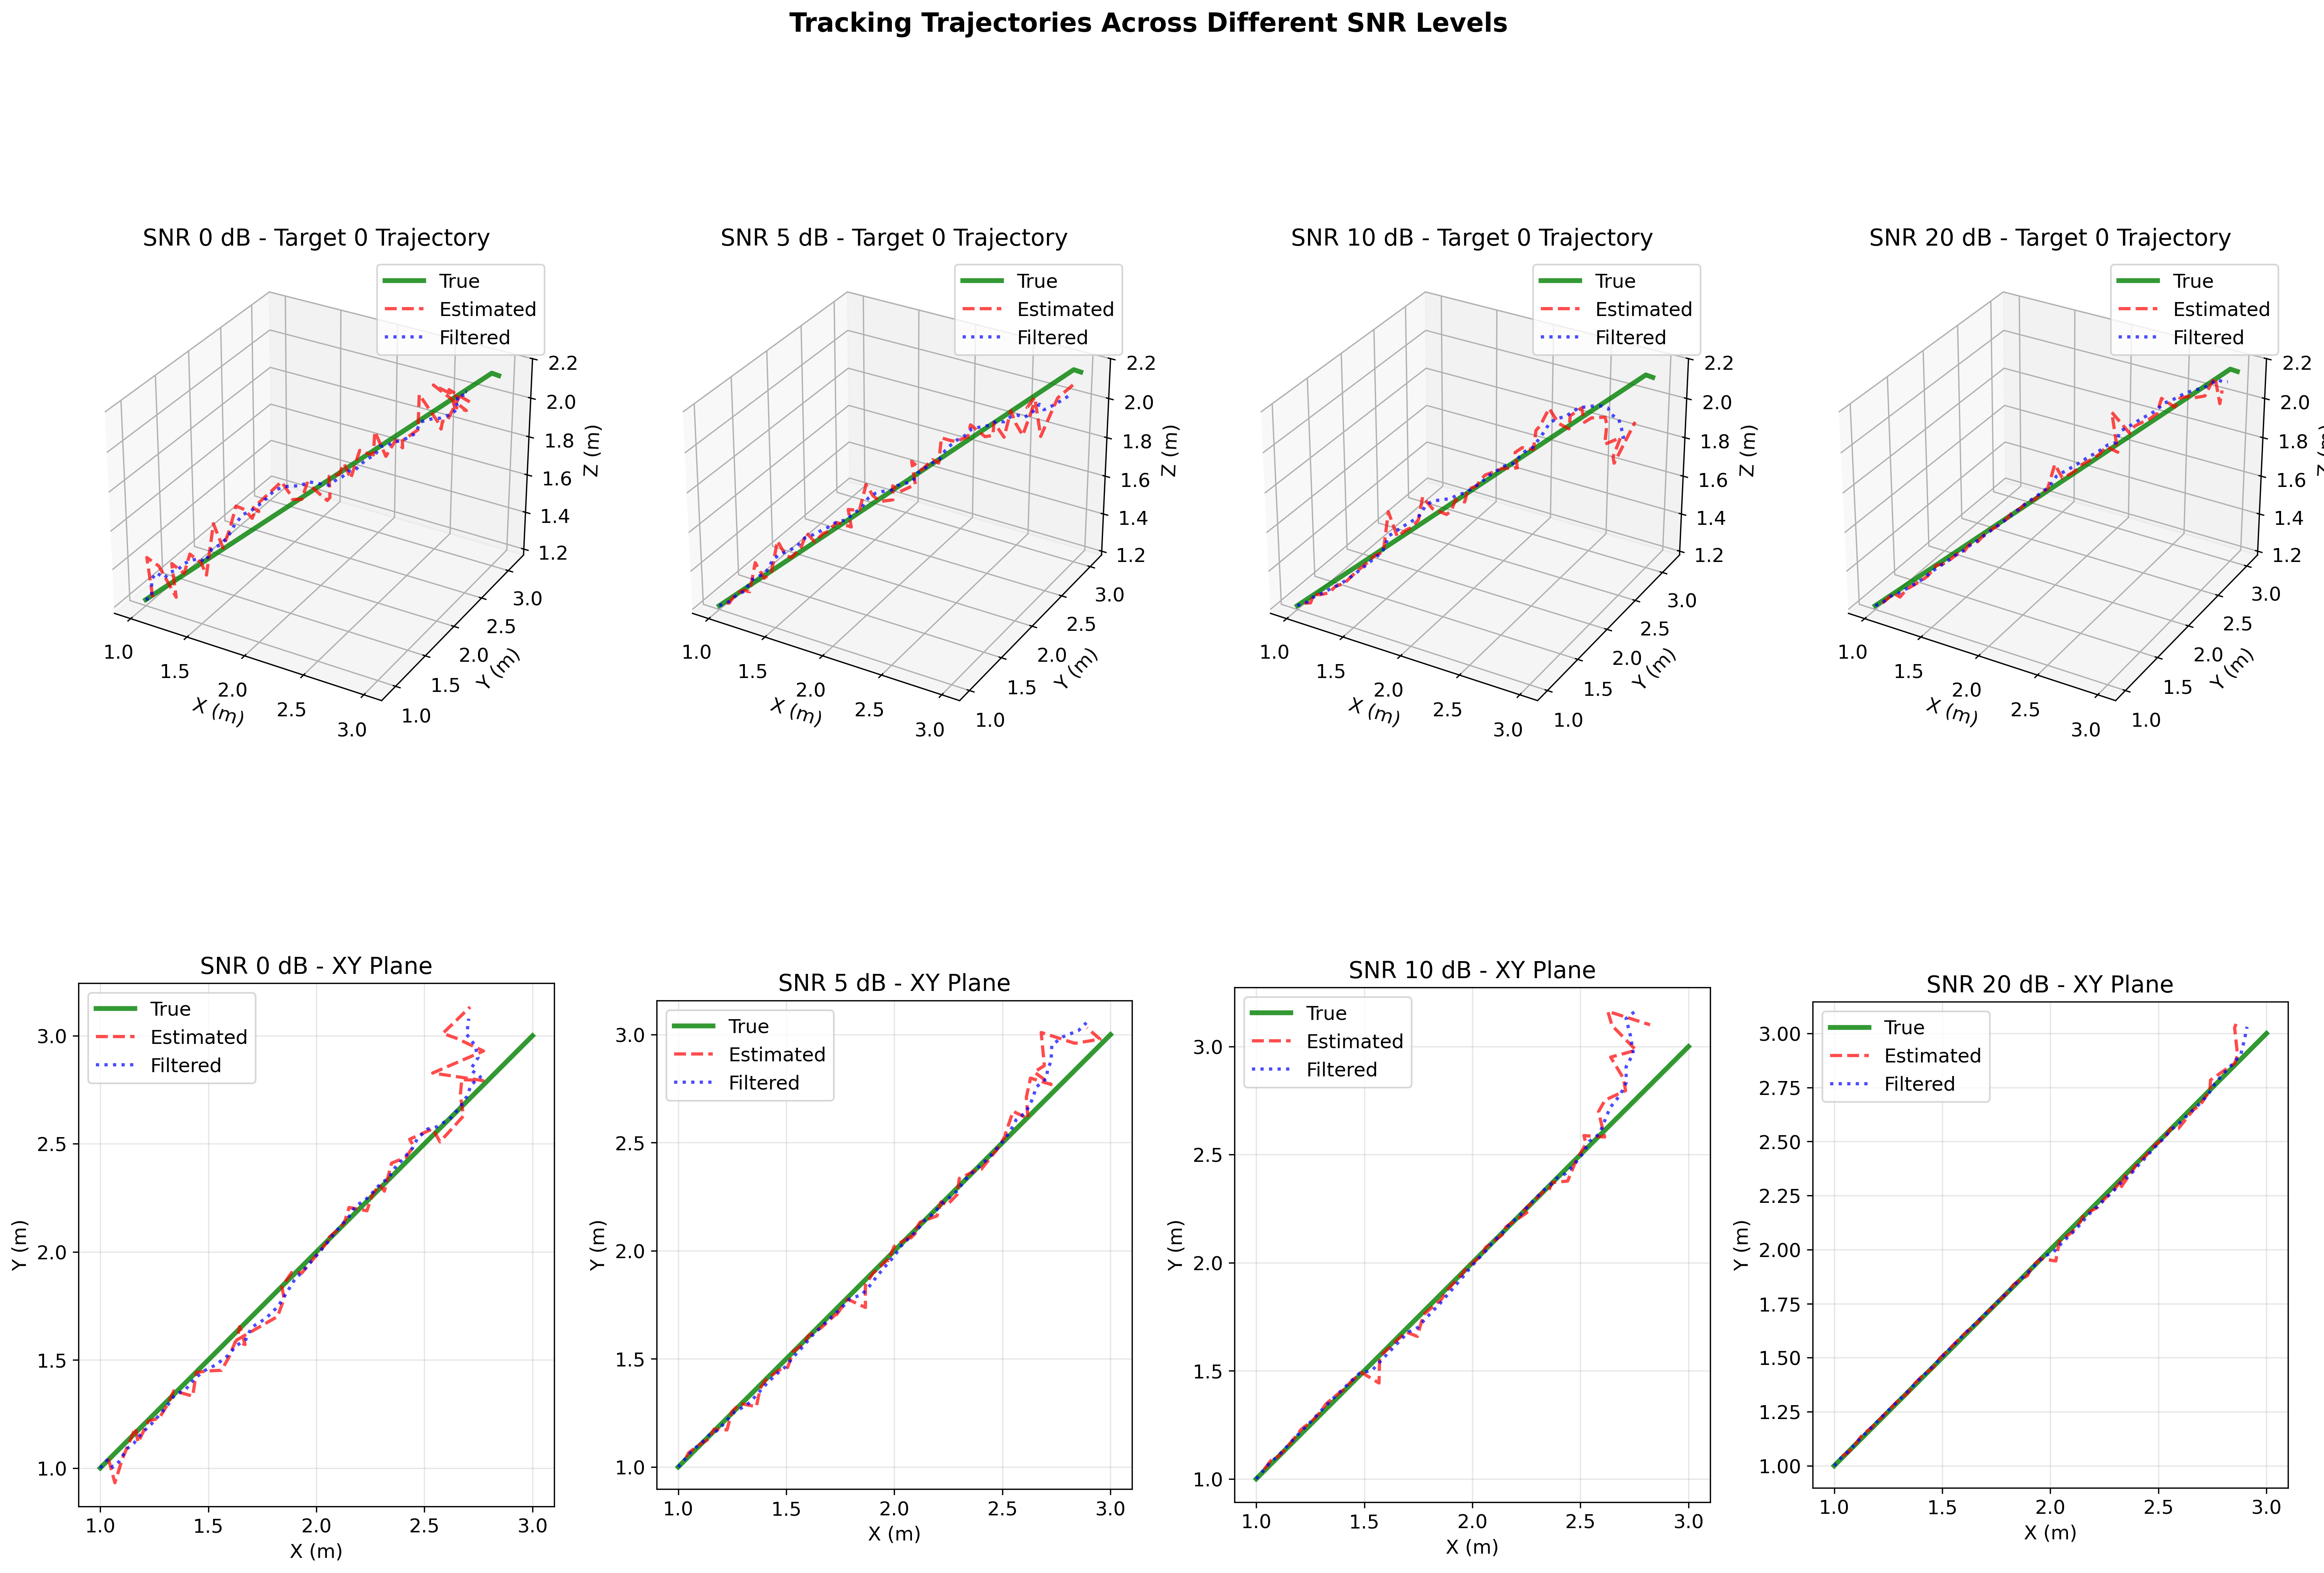
\includegraphics[width=85mm]{final/tracking_trajectories_snr.png}}
\caption{{\it 3D trajectory tracking visualization showing tracked paths across different noise conditions. The results demonstrate successful extension from 2D to 3D tracking with maintained accuracy in all three spatial dimensions.}}
\label{fig:trajectories}
\end{figure}

\section{Challenges and Limitations}

\subsection{Remaining Technical Challenges}

Despite successful 3D extension, several challenges remain:

\begin{itemize}
\item {\em Z-axis precision:} Vertical tracking remains less precise than horizontal tracking
\item {\em Computational overhead:} 9D state vectors and ellipsoid intersections increase processing requirements
\item {\em Array geometry sensitivity:} Performance varies significantly with microphone placement
\item {\em Multipath complexity:} 3D reflections create more complex acoustic environments
\end{itemize}

\subsection{Implementation Limitations}

Current implementation limitations include:

\begin{itemize}
\item {\em Fixed array configurations:} Manual configuration required for different deployments
\item {\em Room-specific calibration:} Acoustic models require environment-specific tuning
\item {\em Target count limitations:} Performance degrades with increased number of simultaneous targets
\end{itemize}

\section{Conclusion}

This work successfully demonstrates the extension of the AMT+ acoustic multi-target tracking system from 2D to full 3D space, addressing fundamental challenges that arise when transitioning from planar to volumetric tracking environments.

\subsection{Technical Contributions}

The key technical achievements in extending AMT+ to 3D include:

\begin{itemize}
\item {\em Enhanced State Modeling:} Successfully expanded from position-only tracking to 9D state vectors to handle 3D position, velocity, and acceleration tracking
\item {\em Two-Stage Multilateration:} Developed adaptive grid search algorithms to handle the computational complexity of multi-ellipsoid intersection problems
\item {\em Z-Axis Stabilization:} Identified and addressed vertical measurement instabilities through adaptive noise modeling and temporal continuity constraints
\item {\em Geometric Constraint Handling:} Implemented solutions for the geometric ambiguities inherent in vertical localization with home theater microphone array configurations
\end{itemize}

\subsection{Challenges Addressed}

The 3D extension required solving several fundamental challenges not present in 2D systems:

{\bf Geometric Ambiguity Resolution:} The limited vertical baseline diversity in typical microphone deployments creates inherent geometric degeneracy. We addressed this through:
\begin{itemize}
\item Adaptive measurement noise covariance that accounts for directional constraints
\item Enhanced z-axis resolution in the multilateration grid search
\item Temporal continuity constraints to prevent unrealistic vertical jumps
\end{itemize}

{\bf Computational Complexity Management:} The transition from 2D ellipse intersections to 3D ellipsoid intersections significantly increases computational requirements. We managed this through:
\begin{itemize}
\item Two-stage adaptive resolution algorithms
\item Trajectory-guided search optimization
\item Ambiguity detection and resolution enhancement
\end{itemize}

{\bf Measurement Stability:} Z-axis measurements exhibit higher uncertainty than horizontal measurements. We handled this through:
\begin{itemize}
\item Directional noise modeling with increased z-axis uncertainty
\item Kalman filter adaptations for 3D motion models
\item Robust estimation techniques for outlier rejection
\end{itemize}

\subsection{Performance Validation}

The AMT3D extension achieves tracking accuracy ranging from 0.095 m to 0.192 m depending on acoustic conditions and array configurations, demonstrating that 3D acoustic tracking is feasible while maintaining practical accuracy levels for real-world applications.

Array configuration analysis reveals:
\begin{itemize}
\item 4-microphone arrays provide approximately 18.2\% better performance than 3-microphone configurations
\item Distributed geometries excel in optimal conditions while compact arrays provide more consistent performance
\item Linear arrangements offer deployment advantages for consumer electronics integration
\end{itemize}

\subsection{Implementation Insights}

Several critical insights emerged during the 3D extension:

\begin{itemize}
\item {\em Z-axis challenges are fundamental:} Vertical positioning remains challenging despite home theater array geometry with some vertical diversity
\item {\em Temporal tracking is essential:} Continuity constraints are crucial for stable 3D tracking, particularly in the vertical dimension
\item {\em Adaptive algorithms are necessary:} Fixed-resolution approaches are insufficient for the varying geometric constraints in 3D space
\end{itemize}

\subsection{Future Research Directions}

The successful 3D extension opens several avenues for future development:

\begin{itemize}
\item {\em Enhanced Array Geometries:} Investigation of vertically-distributed microphone arrays for improved z-axis resolution
\item {\em Machine Learning Integration:} Neural network approaches for handling complex multipath environments and geometric constraints
\item {\em Multi-Scale Tracking:} Extension to larger 3D environments with multiple interconnected spaces
\item {\em Real-Time Optimization:} Further computational efficiency improvements for deployment on resource-constrained devices
\end{itemize}

\subsection{Impact and Applications}

The AMT3D system establishes a foundation for practical 3D acoustic tracking, enabling applications that require full volumetric position awareness:

\begin{itemize}
\item {\em Human Activity Monitoring:} Full-body gesture and movement analysis in 3D space
\item {\em Smart Environment Interaction:} Room-scale interaction systems for smart homes and offices
\item {\em Industrial Applications:} Personnel and equipment tracking in 3D factory environments
\item {\em Assistive Technologies:} Enhanced accessibility interfaces requiring 3D spatial awareness
\end{itemize}

The successful transition from AMT+'s 2D position-only tracking to full 3D motion modeling demonstrates that smartphone-based MIMO systems can be extended to handle the geometric and computational challenges of volumetric environments, providing a foundation for next-generation spatial interaction technologies.

\bibliographystyle{IEEEbib}
\begin{thebibliography}{1}

\bibitem{amt_plus}
P. Wang, R. Jiang, J. Hu, Y. Zhu, H. Jiang, M. Li, and C. Liu,
``AMT+: Acoustic Multi-Target Tracking With Smartphone MIMO System,''
{\em IEEE Transactions on Mobile Computing}, vol. 23, no. 12, pp. 1-14, December 2024.

\bibitem{pyroomacoustics}
R. Scheibler, E. Bezzam, and I. Dokmanić,
``Pyroomacoustics: A Python Package for Audio Room Simulation and Array Processing Algorithms,''
{\em Proc. IEEE International Conference on Acoustics, Speech and Signal Processing (ICASSP)}, pp. 351-355, 2018.

\bibitem{kalman3d}
G. Welch and G. Bishop,
``An Introduction to the Kalman Filter,''
{\em University of North Carolina at Chapel Hill}, Technical Report TR 95-041, 2006.

\end{thebibliography}

\end{document}